\begin{figure}[!htb]
\centering
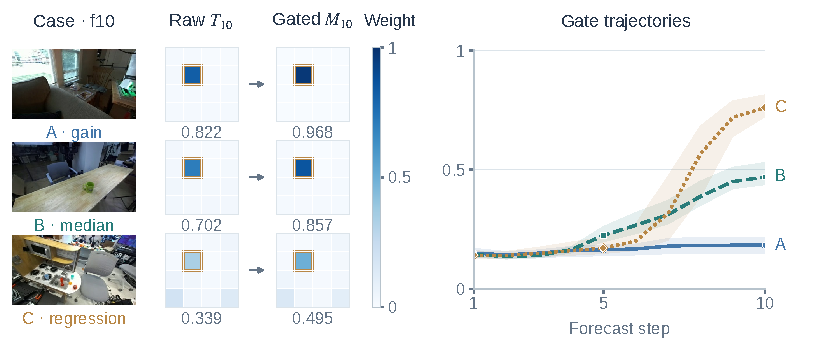
\includegraphics[width=\linewidth]{generated/editorial/mixing_story.pdf}
\caption[Measured spatial mixing and gate behavior.]{\textbf{Measured anchoring and gate trajectories.} A/B/C are the largest-gain, median and largest-regression episodes; each diagnostic uses its first eligible window, as in Figure~\ref{fig:editorial-qualitative}. At target patch $j=5$ (row 2, column 2), maps show raw source weights $T_{10}[j,:]$ and effective weights $M_{10}[j,:]$. $M_h=(1-g_h)I+g_hT_h$ is computed within each seed before averaging. All six maps share a linear $[0,1]$ scale; the amber outline and numbers identify the own-source weight. Gate curves show three-seed means and min--max ranges, not confidence intervals; each forecast step uses five native commands. Full images are recorded $f10$ observations (DROID, CC BY 4.0). These latent-feature diagnostics do not establish physical correspondence or explain error differences causally.}
\label{fig:mixing-diagnostics}
\end{figure}
